\section{问题一的模型建立与求解}

\subsection{半平面交定位模型的建立}

在精准定位阶段，测向机通过比较接收场强的方向变化推断干扰源的方位，并依据多地点的方位读数交会确定干扰源位置。

在使用交会定位法确定干扰源位置时，每个检测点给出指向干扰源的一段允许方向范围，这些方向范围在平面上的公共部分给出仅依据示向度得到的候选位置\textsuperscript{\cite{ref1}}。我们建立``半平面交定位模型''以求解问题。

设第 \(i\) 个检测点坐标为 \(s_i=(x_i,y_i)^{\mathsf T}\)，第 \(i\) 次观测的示向度为 \(\theta_i\)，误差半角为 \(\delta=1^\circ\)，允许方向范围的两条边界方向单位向量记为：
\[
v_i^-=
\begin{pmatrix}\cos(\theta_i-\delta)\\\sin(\theta_i-\delta)\end{pmatrix},
\qquad
v_i^+=
\begin{pmatrix}\cos(\theta_i+\delta)\\\sin(\theta_i+\delta)\end{pmatrix}
\]

其中，\(v_i^-\) 与 \(v_i^+\) 分别为允许方向范围的顺时针边界与逆时针边界，均由检测点指向干扰源前方。

记二维叉积为 \([a,b]=a_xb_y-a_yb_x\)，则单次观测对位置 \(g\) 的约束为：
\[
W_i=\left\{g:\ [v_i^-,g-s_i]\ge0,\quad[v_i^+,g-s_i]\le0\right\}
\tag{1}
\]

将式（1）用坐标展开，得到：
\[
\begin{cases}
\sin(\theta_i-\delta)x-\cos(\theta_i-\delta)y
\le \sin(\theta_i-\delta)x_i-\cos(\theta_i-\delta)y_i,\\[2mm]
-\sin(\theta_i+\delta)x+\cos(\theta_i+\delta)y
\le-\sin(\theta_i+\delta)x_i+\cos(\theta_i+\delta)y_i
\end{cases}
\tag{2}
\]

将全部 \(m\) 次观测的约束联立，得到：
\[
P=\bigcap_{i=1}^{m}W_i
  =\{g\in\mathbb R^2:Ag\le b\}
\tag{3}
\]

其中，\(A\in\mathbb R^{2m\times2}\) 与 \(b\in\mathbb R^{2m}\) 分别由式（2）的系数与右端项按观测顺序组成。 

\subsection{角度交会区域的直径}

\subsubsection{区域直径模型的建立}

对非空有界定位区域 \(P\)，由于半平面是凸集，其交集仍是凸集。区域直径给出其中任意两点之间距离的最大值，我们据此定义``区域直径''：
\[
D(P)=\max_{u,v\in P}\|u-v\|_2
\tag{4}
\]

其中，\(\|\cdot\|_2\) 为欧氏距离。对于非空有界凸多边形，区域直径在有限个顶点对上取得，具体证明如下。

\begin{propositionbox}
\noindent 命题： 设 \(P\) 为非空有界凸多边形，其顶点集为 \(V=\{p_1,\ldots,p_h\}\)，则
\[
D(P)=\max_{1\le i\le j\le h}\|p_i-p_j\|_2
\tag{5}
\]

\noindent 证明： 任取 \(u,v\in P\)，由凸多边形的表示写成
\[
u=\sum_{i=1}^{h}\alpha_i p_i,\qquad
v=\sum_{j=1}^{h}\beta_j p_j,
\quad \alpha_i,\beta_j\ge0,\quad
\sum_i\alpha_i=\sum_j\beta_j=1
\]

其中，\(\alpha_i\)、\(\beta_j\) 为相应的凸组合系数。利用三角不等式，得到
\[
\begin{aligned}
\|u-v\|_2
&=\left\|\sum_{i,j}\alpha_i\beta_j(p_i-p_j)\right\|_2
\le\sum_{i,j}\alpha_i\beta_j\|p_i-p_j\|_2
\le\max_{i,j}\|p_i-p_j\|_2
\end{aligned}
\]

另一方面，所有顶点均属于 \(P\)，故顶点对的最大距离不超过区域直径。两侧合并即得式（5），得证。
\end{propositionbox}

\subsubsection{区域直径模型的求解}

我们采用``半平面求交与顶点枚举算法''以将连续区域上的极值问题化为有限次距离比较，具体步骤如下：

\textbf{Step 1　相容性与有界性判别。} 线性不等式组\(Ag\le b\)可解时，我们分别计算 \(x\) 与 \(y\) 的上、下界，即求解：
\[
\min_{g\in P}x,\qquad\min_{g\in P}(-x),\qquad
\min_{g\in P}y,\qquad\min_{g\in P}(-y)
\tag{6}
\]

四个极值均有限时，\(P\) 被相应的矩形包含而有界；相应的线性规划给出无界性判别。

\textbf{Step 2　半平面求交，构造定位区域顶点集。} 式（3）共给出 \(2m\) 条边界。设第 \(\ell\) 个约束为 \(a_\ell^{\mathsf T}g\le b_\ell\)，我们对所有非平行的边界对 \((\ell,k)\) 求解：
\[
\begin{pmatrix}a_\ell^{\mathsf T}\\a_k^{\mathsf T}\end{pmatrix}z_{\ell k}
=\begin{pmatrix}b_\ell\\b_k\end{pmatrix},
\tag{7}
\]

其中，\(z_{\ell k}\) 为两条边界线的交点。满足全部约束的交点构成候选集 \(\mathcal V=\{z_{\ell k}:Az_{\ell k}\le b\}\)。

我们对候选交点去重，按极角排序以恢复凸多边形的逆时针顶点序列，再沿该顺序剔除位于边上的冗余点，即得顶点 \(p_1,\ldots,p_h\)。

\textbf{Step 3　枚举顶点对，计算区域直径。} 由式（5），我们枚举所有顶点对，得到 \(D(P)\)，同时记录取到最大值的端点 \((p_a,p_b)\)、其中点 \(M\) 与顶点到中点 \(M\) 的最大距离 \(q(P)\)。

\textbf{Step 4　特殊情形处理} 首先判断定位区域 \(P\) 的可行性与有界性：若 \(P=\varnothing\)，则返回``观测不相容''；若 \(P\) 无界，则返回 \(D(P)=+\infty\)。对于非空有界区域，若其退化为单点，则取 \(D(P)=0\)；若其退化为线段，则取两端点之间的距离为区域直径。

\textbf{Step 5　算法参数设置。} 基于本问构型的特点与数值实验，算法参数设置为：交点回代容差 \(10^{-7}\) 米，重复顶点合并距离 \(10^{-6}\) 米，平行边界判据阈值 \(10^{-12}\)，误差半角取题目给定的 \(\delta=1^\circ\)。

上述步骤的求解流程以伪代码记录如下。

\begin{pseudocodetable}
\begin{longtable}{@{}>{\raggedleft\arraybackslash}p{1.8em}@{\hspace{0.65em}}>{\raggedright\arraybackslash}p{\AlgorithmTextWidth}@{}}
\toprule
\multicolumn{2}{@{}p{\linewidth}@{}}{\textbf{算法 1}\quad 半平面求交与顶点枚举算法}\\
\midrule
\multicolumn{2}{@{}p{\linewidth}@{}}{输入：检测点坐标 \(\{s_i\}\)，示向度 \(\{\theta_i\}\)，误差半角 \(\delta\)}\\
\multicolumn{2}{@{}p{\linewidth}@{}}{输出：顶点集 \(V\)，直径 \(D\)，直径端点 \((p_a,p_b)\)，中点 \(M\)，顶点到中点 \(M\) 的最大距离 \(q\)}\\
\endfirsthead
\toprule
\multicolumn{2}{@{}p{\linewidth}@{}}{\textbf{算法 1}\quad 半平面求交与顶点枚举算法（续）}\\
\midrule
\endhead
\midrule
\multicolumn{2}{r}{续下页}\\
\endfoot
\bottomrule
\endlastfoot
\addlinespace[3pt]
1. & \AlgorithmStep{0}{由式(2)构造约束矩阵 \(A\) 与右端项 \(b\)；每次观测产生 \(2\) 个半平面约束}\\
2. & \AlgorithmStep{0}{求解可行性问题 \(Ag\le b\)}\\
3. & \AlgorithmStep{1.2}{若不可行，返回“空集、观测不相容”}\\
4. & \AlgorithmStep{0}{分别求解 \(x\)、\(y\) 的最小值与最大值（式(6)）}\\
5. & \AlgorithmStep{1.2}{若任一极值无界，返回“定位区域无界、\(D=+\infty\)”}\\
6. & \AlgorithmStep{0}{\(V\gets\varnothing\)}\\
7. & \AlgorithmStep{0}{遍历每一对非平行边界 \((\ell,k)\)}\\
8. & \AlgorithmStep{1.2}{由式(7)解出交点 \(z_{\ell k}\)}\\
9. & \AlgorithmStep{1.2}{若 \(Az_{\ell k}\le b\)，则 \(V\gets V\cup\{z_{\ell k}\}\)}\\
10. & \AlgorithmStep{0}{对 \(V\) 去重，按极角排序，剔除边上的冗余点，得顶点集 \(V=\{p_1,\ldots,p_h\}\)}\\
11. & \AlgorithmStep{0}{若 \(h=1\)，令 \(D=0\)，\(p_a=p_b=M=p_1\)，\(q=0\)，返回并按半径 \(0\) 的退化圆处理}\\
12. & \AlgorithmStep{0}{最大平方距离 \(\gets 0\)}\\
13. & \AlgorithmStep{0}{依次取 \(i=1,\ldots,h-1\)}\\
14. & \AlgorithmStep{1.2}{依次取 \(j=i+1,\ldots,h\)}\\
15. & \AlgorithmStep{2.4}{若 \(\lVert p_i-p_j\rVert^2>\) 最大平方距离，则最大平方距离 \(\gets\lVert p_i-p_j\rVert^2\)，\((p_a,p_b)\gets(p_i,p_j)\)}\\
16. & \AlgorithmStep{0}{\(D\gets\sqrt{\text{最大平方距离}}\)，\(M\gets(p_a+p_b)/2\)，\(q\gets\) 各顶点到 \(M\) 的距离最大值}\\
17. & \AlgorithmStep{0}{返回 \(V\)、\(D\)、\((p_a,p_b)\)、\(M\)、\(q\)}\\
\end{longtable}
\end{pseudocodetable}

当前算法的顶点枚举阶段计算复杂度为 \(O(m^3)\)。检测点较多时，可采用方向排序的半平面求交与旋转卡壳法，将主要几何步骤的复杂度降至 \(O(m\log m)\)。复杂度分析与可选优化见附录A。

\subsection{覆盖性的反例检验}

我们构造一个由合法测向约束产生的实例：以区域直径为直径的圆对定位区域的覆盖性在该实例上失效。实例设定三个监测点 \(S'_1\)、\(S'_2\)、\(S'_3\)，其坐标与示向度如表\ref{tab:old2} 所示。

\begingroup
\small
\setlength{\tabcolsep}{4pt}
\setlength{\TableInnerWidth}{\dimexpr\linewidth-8\tabcolsep\relax}
\renewcommand{\arraystretch}{1.22}
\begin{longtable}{@{}>{\centering\arraybackslash}p{0.160\TableInnerWidth}>{\centering\arraybackslash}p{0.210\TableInnerWidth}>{\centering\arraybackslash}p{0.250\TableInnerWidth}>{\centering\arraybackslash}p{0.190\TableInnerWidth}>{\centering\arraybackslash}p{0.190\TableInnerWidth}@{}}
\caption{产生等边三角形定位区域的测向输入}\label{tab:old2}\\
\toprule
监测点 & \(x_i\) / 米 & \(y_i\) / 米 & 示向度 / ° & 误差半角 / ° \\
\midrule
\endfirsthead
\multicolumn{5}{c}{表\thetable\quad 产生等边三角形定位区域的测向输入（续）}\\
\toprule
监测点 & \(x_i\) / 米 & \(y_i\) / 米 & 示向度 / ° & 误差半角 / ° \\
\midrule
\endhead
\midrule
\multicolumn{5}{r}{续下页}\\
\endfoot
\bottomrule
\endlastfoot
\(S'_1\) & -1200 & 0 & 1 & 1 \\
\(S'_2\) & 610 & \(-590\sqrt3\) & 121 & 1 \\
\(S'_3\) & 590 & \(610\sqrt3\) & 241 & 1 \\
\end{longtable}
\endgroup

将表\ref{tab:old2} 中的三组示向度按式（2）转为半平面约束并求交后，交集是一个以40为边长的等边三角形：
\[
A=(-20,0),\quad B=(20,0),\quad C=(0,20\sqrt3),\quad P=\operatorname{conv}\{A,B,C\}
\]

其中，\(P\) 为以 \(A\)、\(B\)、\(C\) 为顶点的三角形定位区域。

对于这一定位区域，\(D(P)=40\) 米。以 \(AB\) 为直径的圆半径为 \(20\) 米，而 \(C\) 到 \(AB\) 中点的距离为 \(20\sqrt3\approx34.641\) 米，顶点 \(C\) 位于该圆之外。其最小包围圆半径为：
\[
\rho(P)=\frac{40}{\sqrt3}\approx23.094\ \text{米}
>\frac{D(P)}2=20\ \text{米}
\]

\begin{figure}[H]
\centering
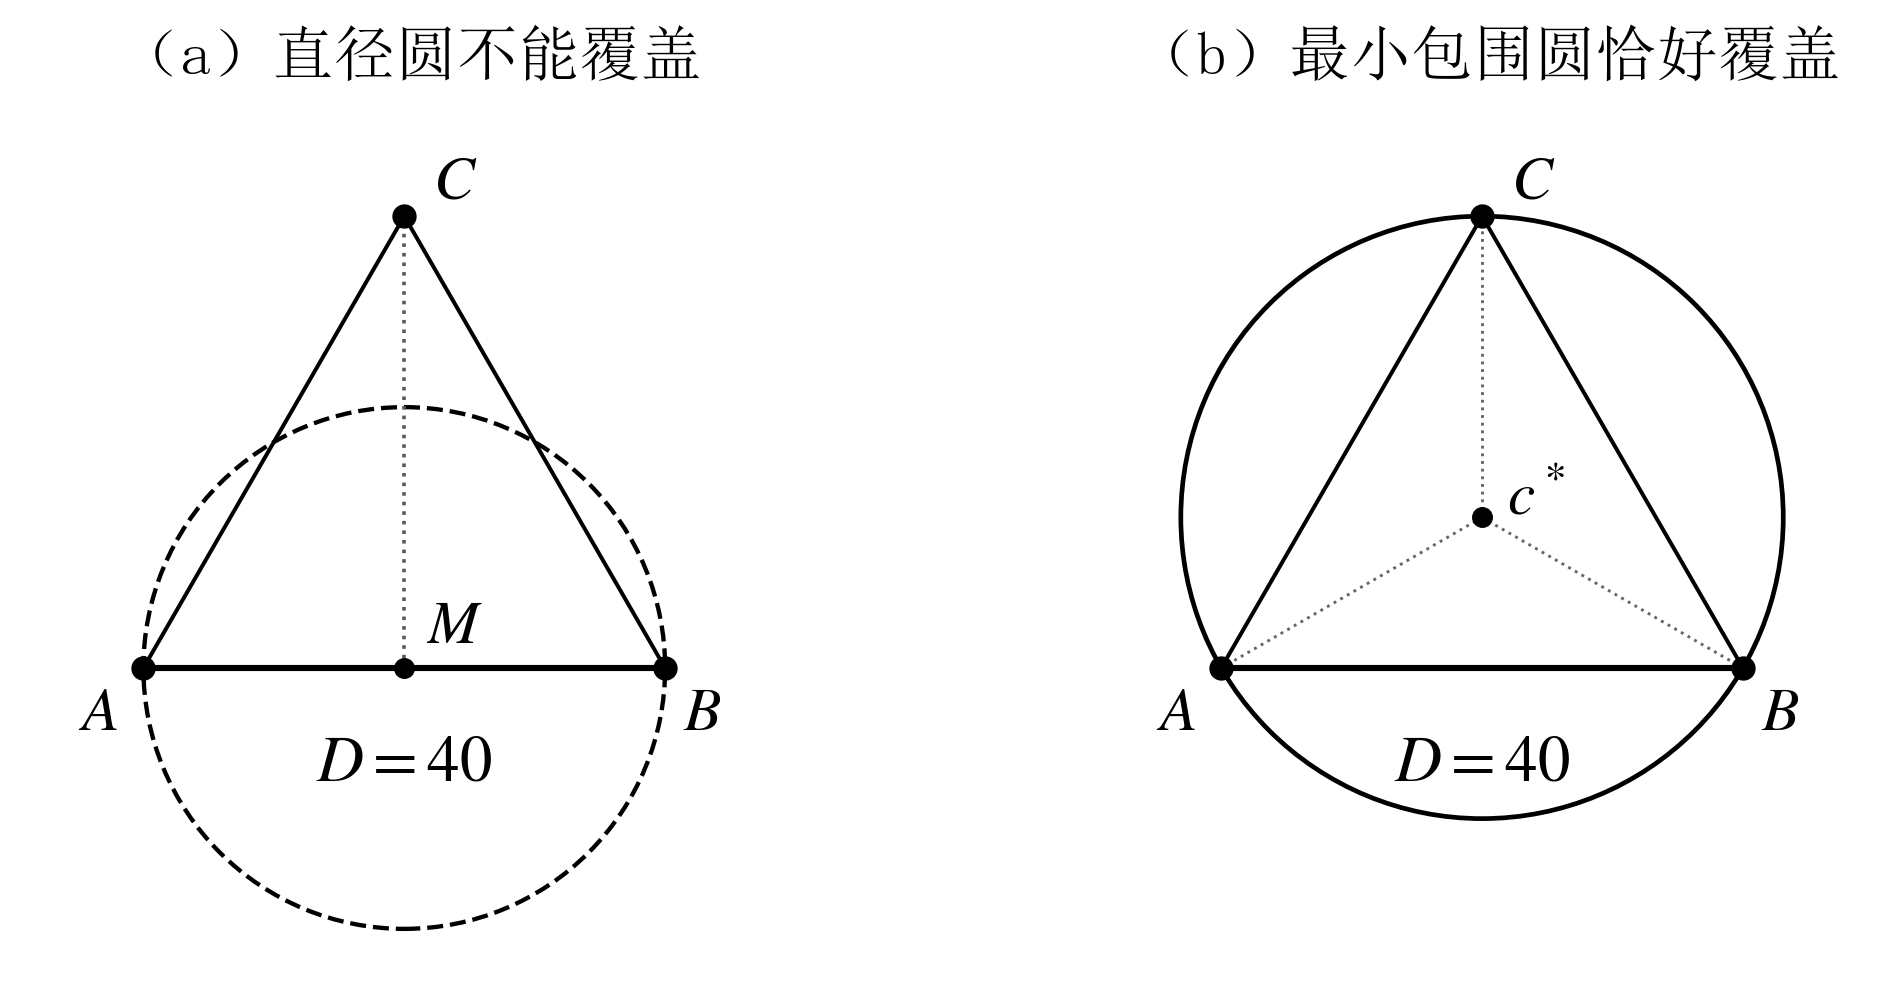
\includegraphics[width=0.84\linewidth,height=0.68\textheight,keepaspectratio]{figures/q1_cover_bw.png}
\caption{等边三角形的直径圆与最小包围圆（长度单位：米）}\label{fig:old1}
\end{figure}

如图\ref{fig:old1} 所示，故以定位区域直径为直径的圆不一定覆盖定位区域。

\subsection{算法准确性与鲁棒性验证}

为检验算法输出的准确性与鲁棒性，我们预先给定干扰源真值 \(G\)，由 \(G\) 与检测点坐标反算真实方向，再按题设误差界生成示向度，构造出定位结果已知的算例。

实例选取四种代表性有界构型：以等边三角形代表一般多边形形态、以线段与单点代表退化形态、以薄多边形代表近退化情形。各实例的构造参数、检测点坐标与示向度如表\ref{tab:old3} 所示。

\begingroup
\renewcommand{\baselinestretch}{1.10}\fontsize{9}{11.5}\selectfont
\setlength{\LTpost}{3pt}
\setlength{\tabcolsep}{4pt}
\setlength{\TableInnerWidth}{\dimexpr\linewidth-6\tabcolsep\relax}
\renewcommand{\arraystretch}{1.05}
\begin{longtable}{@{}>{\centering\arraybackslash}p{0.350\TableInnerWidth}>{\centering\arraybackslash}p{0.340\TableInnerWidth}>{\centering\arraybackslash}p{0.120\TableInnerWidth}>{\centering\arraybackslash}p{0.190\TableInnerWidth}@{}}
\caption{四类实例的构造参数、检测点与示向度}\label{tab:old3}\\
\toprule
实例与构造参数 & 检测点坐标 \(S_i=(x_i,y_i)\) / 米 & 示向度 \(\theta_i\) / ° & 相对真值误差 \(\varepsilon_i\) / ° \\
\midrule
\endfirsthead
\multicolumn{4}{c}{表\thetable\quad 四类实例的构造参数、检测点与示向度（续）}\\
\toprule
实例与构造参数 & 检测点坐标 \(S_i=(x_i,y_i)\) / 米 & 示向度 \(\theta_i\) / ° & 相对真值误差 \(\varepsilon_i\) / ° \\
\midrule
\endhead
\midrule
\multicolumn{4}{r}{续下页}\\
\endfoot
\bottomrule
\endlastfoot
{(a) 三角形　真值 \(G=(0,0)\)；参考圆 \(r=20\) 米；边长 \(20\sqrt3\) 米；测站基距 \(L=1200\) 米} & \parbox[t]{\linewidth}{\centering\setlength{\baselineskip}{14pt}
\rule[-3pt]{0pt}{14pt}\((-1200,-10)\) \\
\rule[-3pt]{0pt}{14pt}\((600+5\sqrt3,\,-600\sqrt3+5)\) \\
\rule[-3pt]{0pt}{14pt}\((600-5\sqrt3,\,600\sqrt3+5)\)
} & \parbox[t]{\linewidth}{\centering\setlength{\baselineskip}{14pt}
\rule[-3pt]{0pt}{14pt}1 \\
\rule[-3pt]{0pt}{14pt}121 \\
\rule[-3pt]{0pt}{14pt}241
} & \parbox[t]{\linewidth}{\centering\setlength{\baselineskip}{14pt}
\rule[-3pt]{0pt}{14pt}+0.522546 \\
\rule[-3pt]{0pt}{14pt}+0.522546 \\
\rule[-3pt]{0pt}{14pt}+0.522546
} \\
\midrule
{(b) 线段　真值 \(G=(50,0)\)；端点 \((0,0)\)、\((100,0)\)；长度 \(100\) 米；参考圆 \(r=50\) 米} & \parbox[t]{\linewidth}{\centering\setlength{\baselineskip}{14pt}
\rule[-3pt]{0pt}{14pt}\((0,0)\) \\
\rule[-3pt]{0pt}{14pt}\((100,0)\)
} & \parbox[t]{\linewidth}{\centering\setlength{\baselineskip}{14pt}
\rule[-3pt]{0pt}{14pt}1 \\
\rule[-3pt]{0pt}{14pt}181
} & \parbox[t]{\linewidth}{\centering\setlength{\baselineskip}{14pt}
\rule[-3pt]{0pt}{14pt}+1.000000 \\
\rule[-3pt]{0pt}{14pt}+1.000000
} \\
\midrule
{(c) 单点　真值 \(G=(0,0)\)；参考圆 \(r=0\)；测站基距 \(L=100\) 米} & \parbox[t]{\linewidth}{\centering\setlength{\baselineskip}{14pt}
\rule[-3pt]{0pt}{14pt}\((-100,0)\) \\
\rule[-3pt]{0pt}{14pt}\((50,-50\sqrt3)\) \\
\rule[-3pt]{0pt}{14pt}\((50,50\sqrt3)\)
} & \parbox[t]{\linewidth}{\centering\setlength{\baselineskip}{14pt}
\rule[-3pt]{0pt}{14pt}1 \\
\rule[-3pt]{0pt}{14pt}121 \\
\rule[-3pt]{0pt}{14pt}241
} & \parbox[t]{\linewidth}{\centering\setlength{\baselineskip}{14pt}
\rule[-3pt]{0pt}{14pt}+1.000000 \\
\rule[-3pt]{0pt}{14pt}+1.000000 \\
\rule[-3pt]{0pt}{14pt}+1.000000
} \\
\midrule
{(d) 薄多边形　真值 \(G=(50,0.0005)\)；高度 \(h=0.001\) 米；对角线横向跨度 \(100\) 米} & \parbox[t]{\linewidth}{\centering\setlength{\baselineskip}{14pt}
\rule[-3pt]{0pt}{14pt}\((0,0)\) \\
\rule[-3pt]{0pt}{14pt}\((100,0.001)\)
} & \parbox[t]{\linewidth}{\centering\setlength{\baselineskip}{14pt}
\rule[-3pt]{0pt}{14pt}1 \\
\rule[-3pt]{0pt}{14pt}181
} & \parbox[t]{\linewidth}{\centering\setlength{\baselineskip}{14pt}
\rule[-3pt]{0pt}{14pt}+0.999427 \\
\rule[-3pt]{0pt}{14pt}+0.999427
} \\
\end{longtable}
\endgroup

\begingroup\renewcommand{\baselinestretch}{1.10}\fontsize{8.5}{11}\selectfont\noindent 注：示向度\(\theta_i\)的取值规则为\(\theta_i=\beta_i+\varepsilon_i\)，其中设检测点 \(S_i\) 指向预设真值 \(G\) 的真实方向为 \(\beta_i\)。\par\endgroup

\begin{figure}[H]
\centering
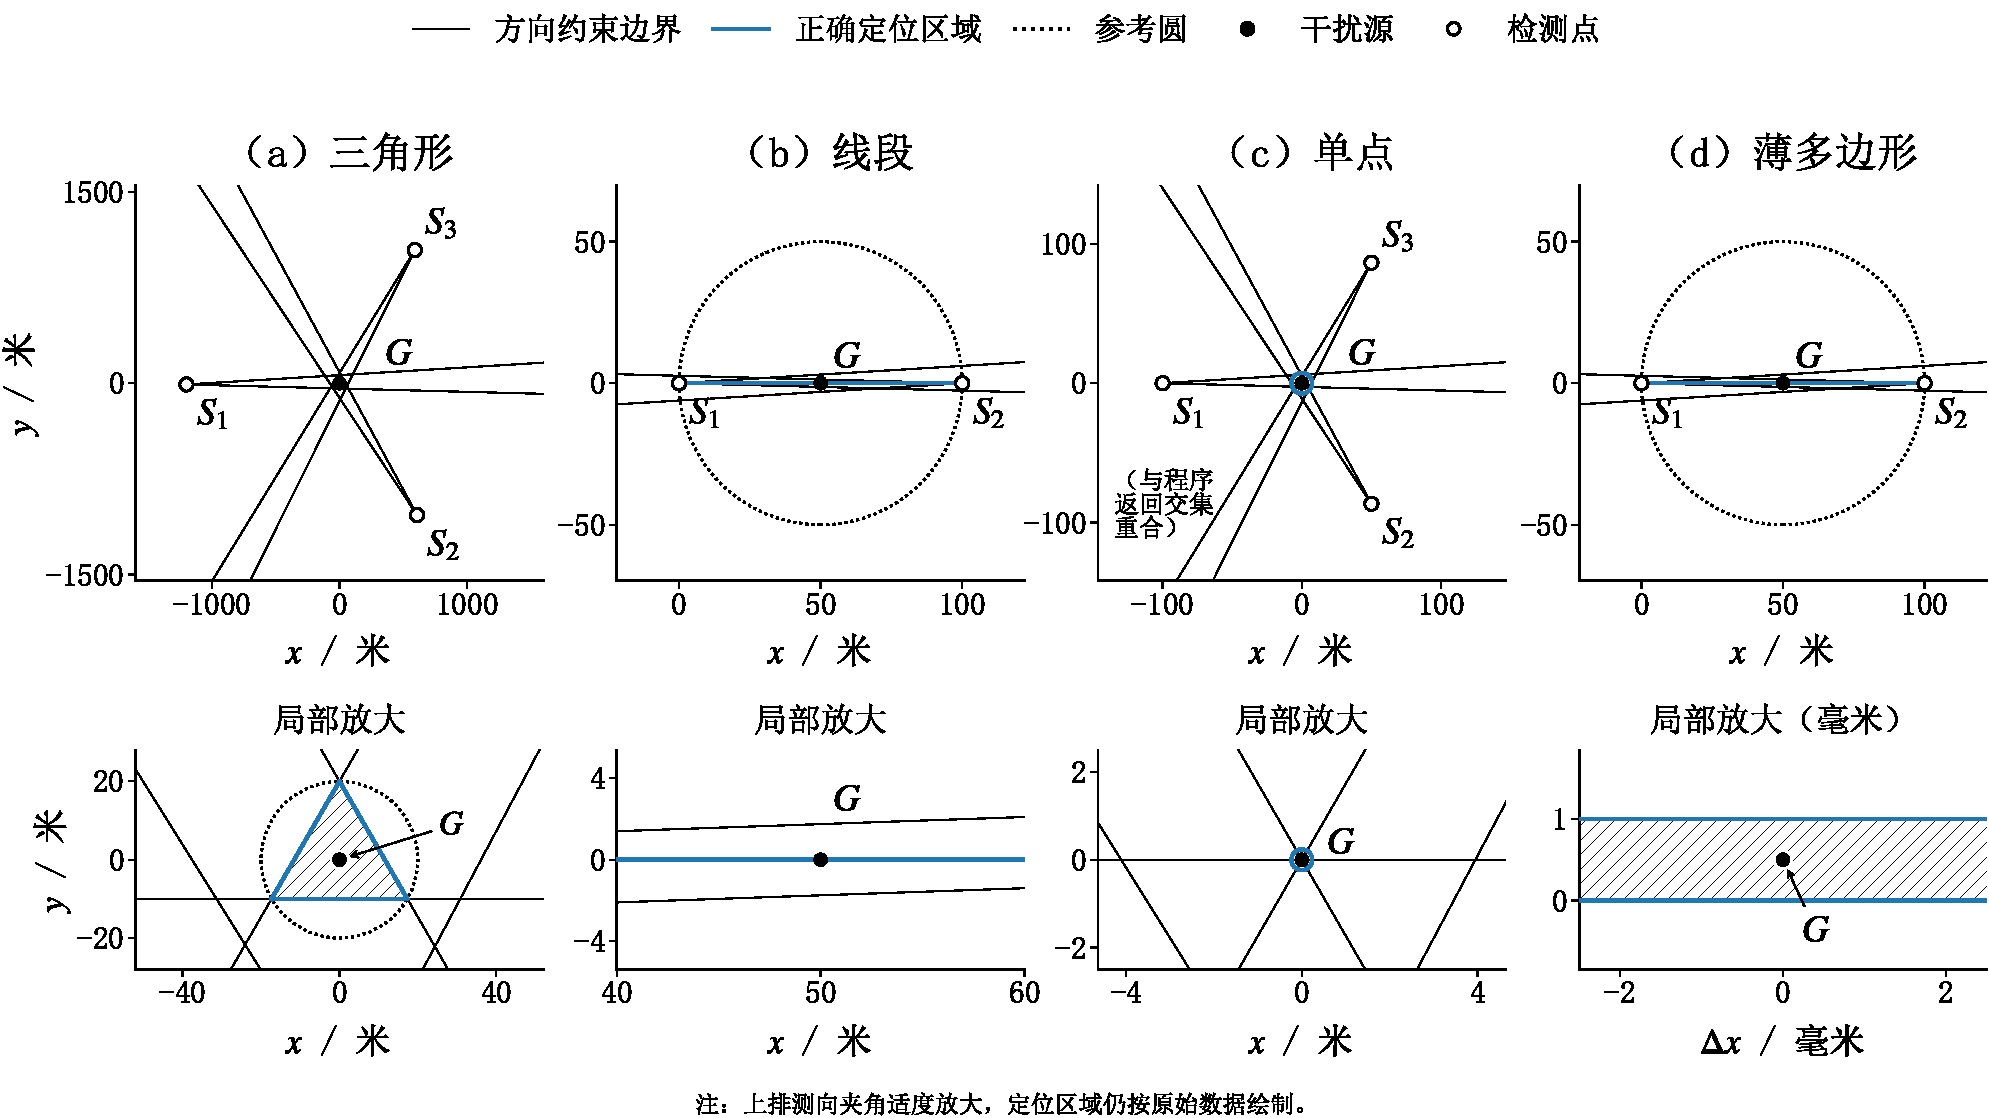
\includegraphics[width=1.00\linewidth,height=0.68\textheight,keepaspectratio]{figures/q1_cases_bw.pdf}
\caption{四类实例的检测点分布与程序返回的定位区域}\label{fig:old2}
\end{figure}

如图\ref{fig:old2}，对每个实例，我们将程序返回的区域类型与顶点集合同预设区域逐一比对，结果发现四类实例在既定数值容差下均与预设区域一致，且预设真值均落入程序返回的定位区域，共同证明了算法具有优秀的准确性与鲁棒性。
